\documentclass{article}

% Packages we used.
\usepackage{graphicx} % Needed for images.
\usepackage{subfig} % For subfigures
\usepackage{amsmath} % Makes math look better usually and provides align/align*

% Title meta-data
\title{MATH340 Day 4 Example}
\author{Hoops and Dr. McNelis}
\date{26 August, 2019}

% This document will contain an example for everything we learned how to do in LaTeX on August 26.

\begin{document}

\maketitle

\section{Images, Again}

% Include a picture, that is 85% of the length of a line.
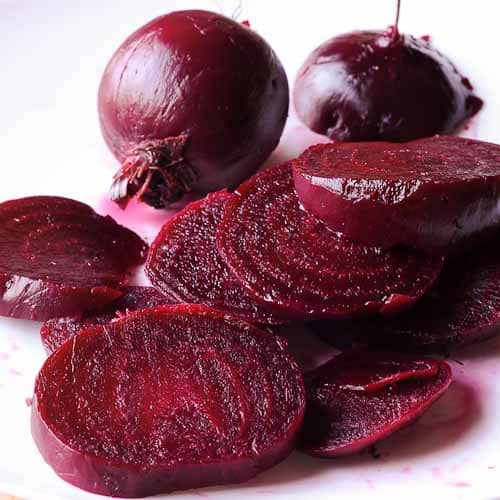
\includegraphics[width=0.25\textwidth]{beets.jpeg} 

% How to make a formal figure. The optional argument comes SECOND and specifies position.
\begin{figure}[h]
    \centering % Makes everything in this environment centered.
    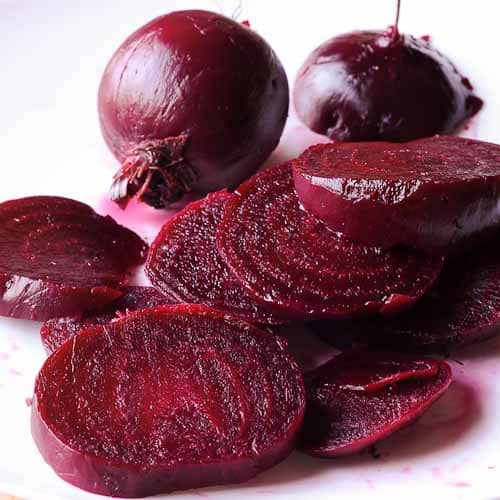
\includegraphics[width=0.15\textwidth]{beets.jpeg} % Puts the actual image in.
    \caption{Caption} % Print a caption here.
    \label{fig:my_label}
\end{figure}

% Positioning:
% [h] = here
% [h!] = HERE!
% [t] = top
% [b] = bottom
% [p] = ? Look it up if you want this one
% You can combine these also, e.g. [htb] = first here, then top if no space, then bottom if no space.

\newpage
\subsection{Subfigures}

\begin{figure}[h!]
    % Use subfloat to make, essentially, a smaller figure within your figure.
    \subfloat[Tilted]{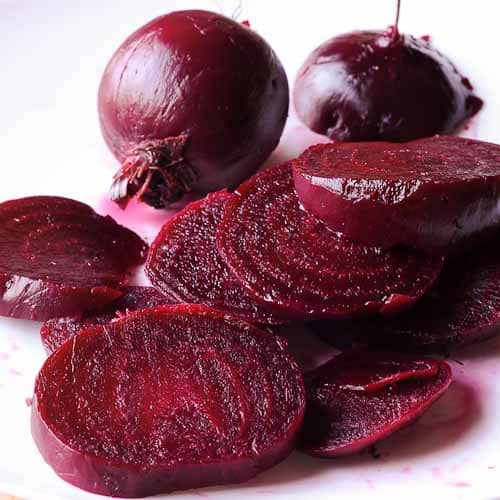
\includegraphics[width=3cm, angle=45]{beets.jpeg} }
    \subfloat[Tilted (the other way)]{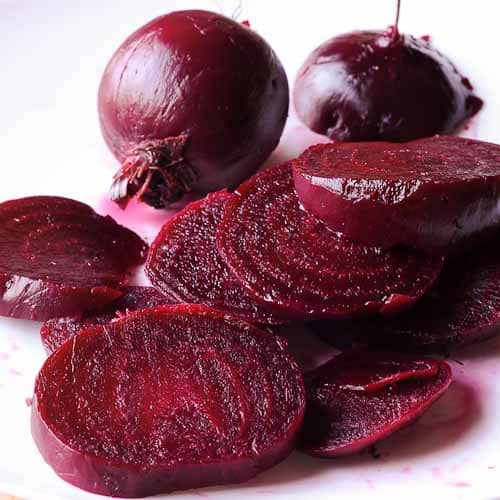
\includegraphics[width=3cm, angle=-45]{beets.jpeg} }
    \caption{Trying out subfigures!}
\end{figure}

\newpage

\section{My First Math}
% How to typeset math statements using LaTeX

% Typesetting inline math--this will be the same height as the sentence it is in. Note that \( ... \) = $ ... $ = \begin{math} ... \end{math} .
My first math in a sentence is to write \( f(x) = \frac{1}{2} \sin(x) - \frac{x+2}{x^2-5} \) is a nifty function.

% Major math equations: typesetting display math which is larger, centered, and looks a lot better. This is an example of how to use align* to line up several equations.

\begin{align*}  %NOTE:  we need \usepackage{amsmath}
    \frac{d}{dx} \left[ \cos \left( e^{x^2} \right) \right] &= \sin \left( e^{x^2} \right) \frac{d}{dx} \left( e^{x^2} \right) \\
    &= -\sin \left( e^{x^2} \right) e^{x^2} \frac{d}{dx} \left( x^2 \right) \\
    &= -\sin \left( e^{x^2} \right) e^{x^2} 2x
\end{align*}


\end{document}
